% Sample file on how to use subfiles.
\documentclass[micro_gen.tex]{subfiles}

\begin{document}

\FloatBarrier

\chapter{Microstructure generation}

In order to conduct numerical analyses of materials with a polycrystalline structure the geometrical properties of the grains in the material must be modeled. Relevant properties to model are the distribution of grain size and the geometrical shape of the grains.
One possibility is to extract the three dimensional microstructure from experiments by using X-ray microtomography. 
The images generated from such an experiment can be analyzed resulting in a digital representation of the microstructure, see for example\cite{Bhandari2007222}.
However, this is a complicated process. The experiments required are extensive and expensive and the post processing of the data is also non trivial. 
 In order to know if the size of the model that is used is large enough for it to be considered an RVE multiple runs have do be performed and the variance in the results have to be evaluated. It can therefore be said that it is necessary to be able to generate different realisations of microstructures of different sizes. Ideally, one would want a mathematically analytic description of a microstructure that is similar enough to the real structure of the material such that a meaningful analysis can be done. One common way of approximating the microstructure in polycrystalline materials is with the Voronoi tesselation. 
 
A Voronoi tessellation is a partition of a domain $D \in \mathbb{R}^d$ into $n$ regions $R_i$ in $D$, each corresponding to one of $n$ different \textit{seed points} $\vec{P}_i$. 
These regions consists of the set of all points that are closer to a particular seed point than to any other,
%
\[R_i = \{ \vec{x} \in D : \left|\left| \vec{P}_i - \vec{x} \right|\right| < \left|\left| \vec{P}_j - \vec{x} \right|\right| \quad  \forall i \neq j, \quad i,j = 1, \ldots, n \}. \]
%
In this thesis the norm used is the Euclidean distance, the dimension of the space is 3 and the bounding domain is a cube.
In this case, the resulting regions will have the shape of convex polyhedrons which are referred to as \textit{grains}. 
This is the grain structure that would exist in a material that forms in the following way:
\begin{itemize}
\item Grains start to nucleate at all the seed points at the same time.
\item The grains grow in all directions at the same rate.
\item A grain boundary is created where the grains meet.
\end{itemize}
In such a Voronoi tesselation two grains will intersect over a plane called a \textit{face},
three grains will intersect along a line called an \textit{edge} and four grains will intersect in a point called a \textit{vertex}. A common way to set the locations of the seed points is to randomly assign them to different positions in $D$. This is known as a \textit{Poisson-Voronoi tesselation}. One extra requirement that can be used is that 
%
\[ \min \left( |\vec{P}_i - \vec{P}_j| \right) < d, \quad \forall i \neq j, \quad d \in \mathbb{R}^+ \]
%
This means that two seed points must at least be separated by a distance $d$. This is called \textit{hardcore Voronoi tessellation}. The physical interpretation of this is that two grains can not start nucleate arbitrarily close to each other. This is however not used in this thesis. An example of a tessellation that has been obtained can be seen in figure \ref{fig:pois_voronoi} where 100 seed points have been used. A comparison between a cross section of a Voronoi tessellation and a polycrystalline material can be seen in figure \ref{fig:slice}.


\begin{figure}[htpb!]
\centering
\begin{subfigure}[b]{.5\textwidth}
  \centering
  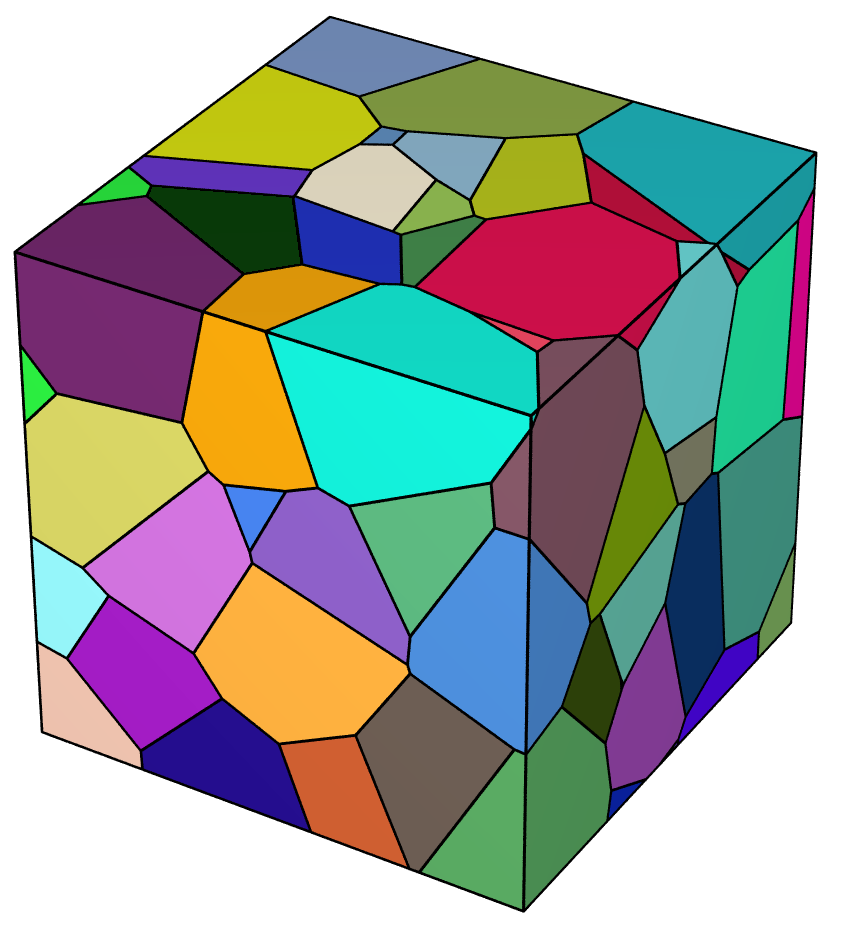
\includegraphics[width=.5\linewidth]{./figures/img_body.png}
  \caption{All polyhedrons shown.}
  \label{fig:pois_voronoi_a}
\end{subfigure}%
\begin{subfigure}[b]{.5\textwidth}
  \centering
  \includegraphics[width=.5\linewidth]{./figures/img_nobody.png}
  \caption{Polyhedrons that are completely inside the domain.}
  \label{fig:pois_voronoi_b}
\end{subfigure}
\caption{Voronoi tessellation containing 100 polyhedrons bounded by a cube}
\label{fig:pois_voronoi}
\end{figure}


 The actual generation of the tessellation can easily be done in for example the commonly used software MATLAB \cite{matlab:voronoi}. The computational time required to generate such a tessellation is negligible for any number of grains that would be reasonable for an RVE of a polycrystalline material. In this thesis the open source software Neper \cite{Quey20111729} was used to generate the tessellation since this software also has a module capable of meshing the generated structure.

\begin{figure}[htpb!]
\centering
\begin{subfigure}[b]{.5\textwidth}
  \centering
  \includegraphics[width=.7\linewidth]{./figures/100_slice.png}
  \caption{}
   \label{fig:slice_a}
\end{subfigure}%
\begin{subfigure}[b]{.5\textwidth}
  \centering
  \includegraphics[width=.5\linewidth]{./figures/CrystalGrain.jpg}
  \caption{}
  \label{fig:slice_b}
\end{subfigure}
\caption{a) Slice through a voronoi tesselation.  b) Micrograph image of a polycrystalline metal.\cite{wiki:grain}}
\label{fig:slice}
\end{figure}


\end{document}
